\begin{enumerate}[1.]
  \item
    \begin{enumerate}[1.]
      \item Sei
        $x = \begin{pmatrix} f_H\\ f_B\\ \ell_H\\ \ell_B \end{pmatrix} \in {\{0, 1\}}^4$
        mit
        \begin{description}
          \item[$f_H$] Fabrikbau in Hamburg
          \item[$f_B$] Fabrikbau in Berlin
          \item[$\ell_H$] Lagerhalle in Hamburg
          \item[$\ell_B$] Lagerhalle in Berlin
        \end{description}
        der gesuchte Lösungsvektor. Die Nebenbedingungen ergeben sich aus
        folgender Ungleichung:
        \begin{align*}
          \begin{pmatrix}
            1  & 1  &    & \\
               &    & 1  & 1\\
            -1 & -1 &    & \\
               & -1 &    & 1\\
            -1 &    & 1  & \\
            1  &    &    & \\
            -1 &    &    & \\
               & 1  &    & \\
               & -1 &    & \\
               &    & 1  & \\
               &    & -1 & \\
               &    &    & 1\\
               &    &    & -1\\
            6  & 3  & 5  & 2
          \end{pmatrix}
          \begin{pmatrix}
            f_H\\
            f_B\\
            \ell_H\\
            \ell_B
          \end{pmatrix}
          \leq
          \begin{pmatrix}
            2\\
            1\\
            -1\\
            0\\
            0\\
            1\\
            0\\
            1\\
            0\\
            1\\
            0\\
            1\\
            0\\
            10
          \end{pmatrix}
        \end{align*}
        Die zu maximierende Zielfunktion lautet
        \begin{align*}
          f(f_H, f_B, \ell_H, \ell_B) = 9 f_H + 5 f_B + 6 \ell_H + 4 \ell_B
        \end{align*}
        also ist $c = \begin{pmatrix}
          9\\
          5\\
          6\\
          4
        \end{pmatrix}$.

      \pagebreak

      \item Die Informationen eines Knotens im Ableitungsbaum seien wie folgt
        kodiert:
        \begin{center}
          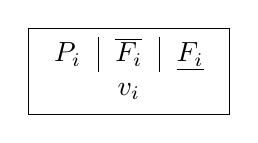
\begin{tikzpicture}[scale=1]
            \node [draw] {%
              \begin{tabular}{l|c|c}
                $P_i$
                & $\overline{F_i}$
                & $\underline{F_i}$\\
                \midrule
                \multicolumn{3}{c}{%
                  $v_i$
                }
              \end{tabular}
            };
          \end{tikzpicture}
        \end{center}
        Damit ergibt sich folgender Ableitungsbaum:
        \begin{center}
          \begin{tikzpicture}[
              scale=1,
              level distance=35mm,
              level 1/.style={sibling distance=45mm},
              level 2/.style={sibling distance=80mm},
              level 3/.style={sibling distance=40mm},
              every child node/.style={draw}
          ]
            \node [draw] {%
              \begin{tabular}{l|c|c}
                $P_1$
                & $16{,}5$
                & $0$\\
                \midrule
                \multicolumn{3}{c}{%
                  $\begin{pmatrix}
                    0{,}8 & 1 & 0 & 1
                  \end{pmatrix}$
                }
              \end{tabular}
            }
              child {%
                node {%
                  \begin{tabular}{l|c|c}
                    $P_2$
                    & $9$
                    & $9$\\
                    \midrule
                    \multicolumn{3}{c}{%
                      $\begin{pmatrix}
                        0 & 1 & 0 & 1
                      \end{pmatrix}$
                    }
                  \end{tabular}
                }
                edge from parent node [near end, above left] {$f_H = 0$}
              }
              child {%
                node {%
                  \begin{tabular}{l|c|c}
                    $P_3$
                    & $16{,}2$
                    & $9$\\
                    \midrule
                    \multicolumn{3}{c}{%
                      $\begin{pmatrix}
                        1 & 0{,}8 & 0 & 0{,}8
                      \end{pmatrix}$
                    }
                  \end{tabular}
                }
                child {%
                  node {%
                    \begin{tabular}{l|c|c}
                      $P_4$
                      & $13{,}8$
                      & $9$\\
                      \midrule
                      \multicolumn{3}{c}{%
                        $\begin{pmatrix}
                          1 & 0 & 0{,}8 & 0
                        \end{pmatrix}$
                      }
                    \end{tabular}
                  }
                  child {%
                    node {%
                      \begin{tabular}{l|c|c}
                        $P_5$
                        & $9$
                        & $9$\\
                        \midrule
                        \multicolumn{3}{c}{%
                          $\begin{pmatrix}
                            1 & 0 & 0 & 0
                          \end{pmatrix}$
                        }
                      \end{tabular}
                    }
                    edge from parent node [near end, above left] {$\ell_H = 0$}
                  }
                  child {%
                    node {%
                      \begin{tabular}{l|c|c}
                        $P_6$ & \multicolumn{2}{c}{$\emptyset$}\\
                        \midrule
                        \multicolumn{3}{c}{%
                          Keine opt. Lösung.
                        }
                      \end{tabular}
                    }
                    edge from parent node [near end, above right] {$\ell_H = 1$}
                  }
                  edge from parent node [near end, above left] {$f_B = 0$}
                }
                child {%
                  node {%
                    \begin{tabular}{l|c|c}
                      $P_7$
                      & $16$
                      & $9$\\
                      \midrule
                      \multicolumn{3}{c}{%
                        $\begin{pmatrix}
                          1 & 1 & 0 & 0{,}5
                        \end{pmatrix}$
                      }
                    \end{tabular}
                  }
                  child {%
                    node {%
                      \begin{tabular}{l|c|c}
                        $P_8$
                        & $15{,}2$
                        & $9$\\
                        \midrule
                        \multicolumn{3}{c}{%
                          $\begin{pmatrix}
                            1 & 1 & 0{,}2 & 0
                          \end{pmatrix}$
                        }
                      \end{tabular}
                    }
                    child {%
                      node {%
                        \begin{tabular}{l|c|c}
                          $P_9$
                          & $14$
                          & $9$\\
                          \midrule
                          \multicolumn{3}{c}{%
                            $\begin{pmatrix}
                              1 & 1 & 0 & 0
                            \end{pmatrix}$
                          }
                        \end{tabular}
                      }
                      edge from parent node [near end, above left] {$\ell_H = 0$}
                    }
                    child {%
                      node {%
                        \begin{tabular}{l|c|c}
                          $P_{10}$ & \multicolumn{2}{c}{$\emptyset$}\\
                          \midrule
                          \multicolumn{3}{c}{%
                            Keine opt. Lösung.
                          }
                        \end{tabular}
                      }
                      edge from parent node [near end, above right] {$\ell_H = 1$}
                    }
                    edge from parent node [near end, above left] {$\ell_B = 0$}
                  }
                  child {%
                    node {%
                      \begin{tabular}{l|c|c}
                        $P_{11}$ & \multicolumn{2}{c}{$\emptyset$}\\
                        \midrule
                        \multicolumn{3}{c}{%
                          Keine opt. Lösung.
                        }
                      \end{tabular}
                    }
                    edge from parent node [near end, above right] {$\ell_B = 1$}
                  }
                  edge from parent node [near end, above right] {$f_B = 1$}
                }
                edge from parent node [near end, above right] {$f_H = 1$}
              };
          \end{tikzpicture}
        \end{center}
        Bei $P_5$ ist die Suche ausgelotet, weil $\overline{F_5} =
        \underline{F_5}$ gilt. Bei $P_6, P_{10}$ und $P_{11}$ ist die Suche
        ausgelotet, weil keine optimale Lösung gefunden wurde.

        Die optimale Lösung ist daher $P_9$, das heißt, dass Fabriken in Hamburg
        und Berlin gebaut werden, auf Lagerhallen jedoch verzichtet wird.

    \end{enumerate}

  \pagebreak

  \item \begin{enumerate}
    \item
      \begin{align*}
        S & \stackrel{(1)}{\rightarrow}
          \texttt{if\textvisiblespace{}condition\textvisiblespace{}then\textvisiblespace{}}SE\\
          & \stackrel{(4)}{\rightarrow}
          \texttt{if\textvisiblespace{}condition\textvisiblespace{}then\textvisiblespace{}}S\texttt{\textvisiblespace{}else\textvisiblespace{}}S\\
          & \stackrel{(1)}{\rightarrow}
          \texttt{if\textvisiblespace{}condition\textvisiblespace{}then\textvisiblespace{}}\texttt{if\textvisiblespace{}condition\textvisiblespace{}then\textvisiblespace{}}SE\texttt{\textvisiblespace{}else\textvisiblespace{}}S\\
          & \stackrel{(2)}{\rightarrow}
          \texttt{if\textvisiblespace{}condition\textvisiblespace{}then\textvisiblespace{}}\texttt{if\textvisiblespace{}condition\textvisiblespace{}then\textvisiblespace{}statement;}E\texttt{\textvisiblespace{}else\textvisiblespace{}}S\\
          & \stackrel{(3)}{\rightarrow}
          \texttt{if\textvisiblespace{}condition\textvisiblespace{}then\textvisiblespace{}}\texttt{if\textvisiblespace{}condition\textvisiblespace{}then\textvisiblespace{}statement;}\texttt{\textvisiblespace{}else\textvisiblespace{}}S\\
          & \stackrel{(2)}{\rightarrow}
          \texttt{if\textvisiblespace{}condition\textvisiblespace{}then\textvisiblespace{}}\texttt{if\textvisiblespace{}condition\textvisiblespace{}then\textvisiblespace{}statement;}\texttt{\textvisiblespace{}else\textvisiblespace{}statement;}
      \end{align*}

    \item Die Ableitung eines Wortes ist nicht immer eindeutig. Das Wort
      \begin{center}
        \texttt{if\textvisiblespace{}condition\textvisiblespace{}then\textvisiblespace{}if\textvisiblespace{}condition\textvisiblespace{}then\textvisiblespace{}statement;\textvisiblespace{}else\textvisiblespace{}statement;}
      \end{center}
      hat zwei verschiedene Ableitungsbäume. Einerseits:
      \begin{center}
        \begin{tikzpicture}[
            scale=1,
            level distance=15mm,
            level 1/.style={sibling distance=50mm},
            level 2/.style={sibling distance=25mm},
            level 3/.style={sibling distance=40mm},
          ]
          \node {$S$}
            child {node {\texttt{if\textvisiblespace{}condition\textvisiblespace{}then\textvisiblespace{}}}}
            child {%
              node {$S$}
              child {node {\texttt{if\textvisiblespace{}condition\textvisiblespace{}then\textvisiblespace{}}}}
              child {%
                node {$S$}
                child {node {\texttt{statement;}}}
              }
              child {%
                node {$E$}
                child
              }
            }
            child {%
              node {$E$}
              child {node {\texttt{\textvisiblespace{}else\textvisiblespace{}}}}
              child {%
                node {$S$}
                child {node {\texttt{statement;}}}
              }
            }
          ;
        \end{tikzpicture}
      \end{center}
      Andererseits:
      \begin{center}
        \begin{tikzpicture}[
            scale=1,
            level distance=15mm,
            level 1/.style={sibling distance=50mm},
            level 2/.style={sibling distance=25mm},
            level 3/.style={sibling distance=10mm},
            level 4/.style={sibling distance=10mm},
          ]
          \node {$S$}
            child {node {\texttt{if\textvisiblespace{}condition\textvisiblespace{}then\textvisiblespace{}}}}
            child {%
              node {$S$}
              child {node {\texttt{if\textvisiblespace{}condition\textvisiblespace{}then\textvisiblespace{}}}}
              child {%
                node {$S$}
                child {node {\texttt{statement;}}}
              }
              child {%
                node {$E$}
                child {node {\texttt{\textvisiblespace{}else\textvisiblespace{}}}}
                child {%
                  node {$S$}
                  child {node {\texttt{statement;}}}
                }
              }
            }
            child {%
              node {$E$}
              child
            }
          ;
        \end{tikzpicture}
      \end{center}
      Damit ist die Grammatik mehrdeutig. Das liegt daran, dass die rechte Seite
      der Regel $E \rightarrow \varepsilon$ ein Präfix der rechten Seite der
      Regel $E \rightarrow \texttt{\textvisiblespace{}else\textvisiblespace{}}S$
      ist.
  \end{enumerate}

  \pagebreak

  \item
    \begin{enumerate}[(a)]
      \item Sei $G = (X,H,R,S)$ mit
        \begin{align*}
          X & = \{a, b, c\}\\
          H & = \{S, A, B, C\}\\
          R & = \{
            (S, \varepsilon), (S, ABC),\\
            & \phantom{=}\quad (AB, BA), (BA, AB),\\
            & \phantom{=}\quad (AC, CA), (CA, AC),\\
            & \phantom{=}\quad (BC, CB), (CB, BC),\\
            & \phantom{=}\quad (A, AABC), (B, BABC), (C, CABC),\\
            & \phantom{=}\quad (A, a), (B, b), (C, c)\}
        \end{align*}

      \item
        \begin{align*}
          S & \rightarrow ABC \rightarrow ACB \rightarrow ACABCB\\
          & \rightarrow aCABCB \rightarrow acABCB \rightarrow acaBCB
            \rightarrow acabCB \rightarrow acabcB \rightarrow acabcb
        \end{align*}

      \item Die Grammatik ist längenmonoton, weil einerseits für alle
        $(l, r) \in R$ mit $l \neq S$ die Eigenschaft $|l| \leq |r|$
        gilt, und andererseits, da $(S, \varepsilon) \in R$, das
        Nichtterminal $S$ auf keiner rechten Seite in $R$ vorkommt.
    \end{enumerate}
\end{enumerate}
